\documentclass[tikz,border=8pt]{standalone}
% Shared look for every TikZ diagram. Load with \input{../../tools/tikz-style.tex}
\usepackage[T1]{fontenc}
\usepackage{lmodern}
\renewcommand{\sfdefault}{lmr}  % diagrams use the same serif as the text
\usetikzlibrary{arrows.meta, positioning, shapes.geometric, calc, fit, backgrounds}
\definecolor{cblue}{HTML}{4C78A8}
\definecolor{corange}{HTML}{F58518}
\definecolor{cgreen}{HTML}{54A24B}
\definecolor{cred}{HTML}{E45756}
\definecolor{cpurple}{HTML}{B279A2}
\definecolor{cgrey}{HTML}{6B6B6B}
\tikzset{
  every picture/.style={font=\sffamily, line width=1.2pt},
  box/.style={draw=#1, fill=#1!12, rounded corners=4pt, align=center, inner sep=7pt, minimum height=1.1cm},
  box/.default=cgrey,
  arrow/.style={-{Stealth[length=3mm]}, draw=cgrey, line width=1.4pt},
  title/.style={font=\sffamily\bfseries\Large},
  note/.style={font=\sffamily\small, text=cgrey, align=center},
}
\AtBeginDocument{\hyphenpenalty=10000 \exhyphenpenalty=10000}

\begin{document}
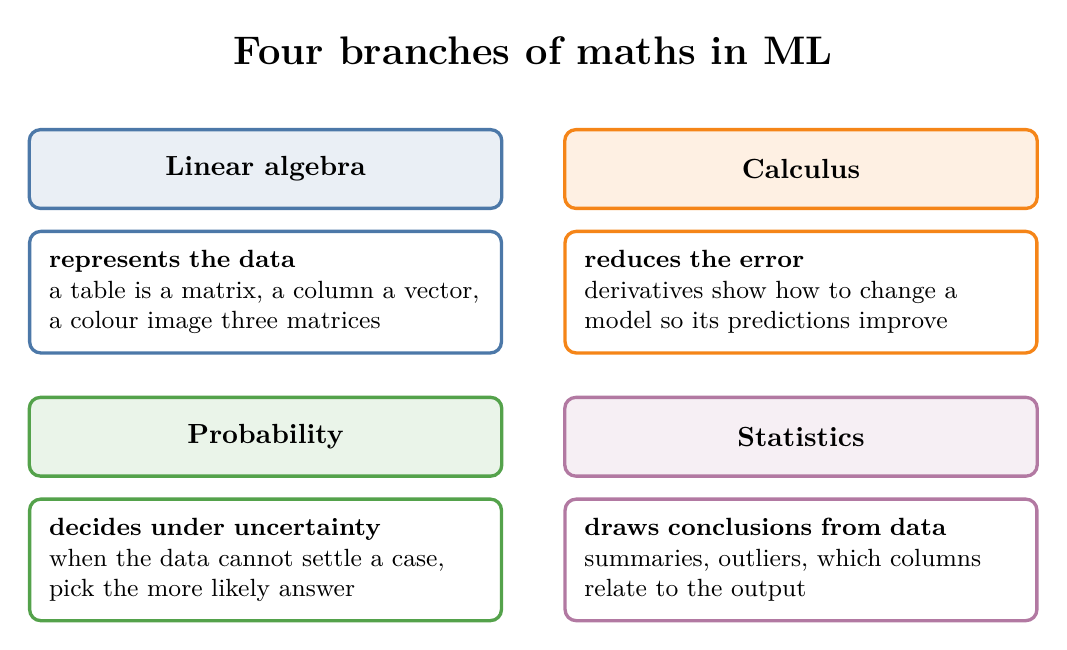
\begin{tikzpicture}[
  br/.style={box=#1, font=\sffamily\bfseries, minimum width=6cm, minimum height=1cm},
  job/.style={draw=#1, fill=white, rounded corners=4pt, align=left, inner sep=7pt, text width=5.5cm, font=\sffamily\small},
]
  \node[title] at (3.4,1.5) {Four branches of maths in ML};

  \node[br=cblue] (la) at (0,0) {Linear algebra};
  \node[job=cblue, below=0.25cm of la] (lat) {\textbf{represents the data}\\ a table is a matrix, a column a vector,\\ a colour image three matrices};

  \node[br=corange] (ca) at (6.8,0) {Calculus};
  \node[job=corange, below=0.25cm of ca] (cat) {\textbf{reduces the error}\\ derivatives show how to change a\\ model so its predictions improve};

  \node[br=cgreen] (pr) at (0,-3.4) {Probability};
  \node[job=cgreen, below=0.25cm of pr] (prt) {\textbf{decides under uncertainty}\\ when the data cannot settle a case,\\ pick the more likely answer};

  \node[br=cpurple] (st) at (6.8,-3.4) {Statistics};
  \node[job=cpurple, below=0.25cm of st] (stt) {\textbf{draws conclusions from data}\\ summaries, outliers, which columns\\ relate to the output};
\end{tikzpicture}
\end{document}
